\documentclass[../main.tex]{subfiles}
\begin{document}

\tikzstyle{block} = [draw, rectangle, text width=2cm, text centered, minimum height=1.2cm, node distance=3cm]
\tikzstyle{bigblock} = [draw, rectangle, text width=2cm, text centered, minimum height=2.2cm, minimum width=3.2cm, node distance=3cm]
\tikzstyle{container} = [draw, rectangle, inner sep=0.3cm]


\section{Introduction}
In the following chapter the theory behind compiler and the build process is introduced. At the end a introduction over the Sconc build framework is reported. The Scons framework is the basic structure upon which the generation of Ecu code is based. 

\section{Compiler}
A compiler is a complex machine that bridges the gap between human readable code and computer readable code.\\
In a model based manner the compiler takes as input source code in a high-level programming language (such as C, C++, Python) and return as a output code in a low level language that compose the executable program. 
\begin{figure}[h]
  \centering
\begin{tikzpicture}
    \node [block, name=text1] {Source code};
    \node [block, right of=text1] (text2) {Front End};
    \node [block, right of=text2] (text3) {Middle End};
    \node [block, right of=text3] (text4) {Back end};
    \node [block, right of=text4] (text5) {Executable code};
    \node [container,fit=(text2) (text3) (text4)] (container) {};

    \draw [->] (text1) -- (text2);
    \draw [->] (text2) -- node {} (text3);
    \draw [->] (text3) -- node {} (text4);
    \draw [->] (text4) -- node {} (text5);
\end{tikzpicture}
  \caption{Compiler overview structure}
\end{figure}
In a executable program generated by the compiler we find a list of instruction to follow all written in binary (machine code). The instruction in binary code are needed to connect together the correct circuits in the CPU, by mean of activating (1) ore deactivating (0) certain transistors, and therefor completing the instructions. Since the CPU can only perform operation such as memory read-wright and basic math the compiler does not only need to translate the source code in binary code, but has also to execute a series of operation to adapt the complexity to the CPU. 
The main components of a compiler are the following:
\begin{itemize}
    \item The front end;
    \item The middle end;
    \item The back end. 
\end{itemize}
In order to better visualize the concepts, consider the following example, based on \cite{frametheessence}. 
  \begin{lstlisting}[language=C]
int main() {
   int x;
   x = 3;
}
  \end{lstlisting}
\begin{figure}[h]
  \centering
\begin{tikzpicture}
    \node [block, name=text1] {Source code};
    \node [block, right of=text1] (text2) {Scanning};
    \node [block, right of=text2] (text3) {Parsing};
    \node [block, right of=text3] (text4) {Semantics analysis};
    \node [block, right of=text4] (text5) {IR gen.};
    \node [block, right of=text5] (text6) {IR};
    \node [container,fit=(text2) (text3) (text4) (text5)] (container) {};

    \draw [->] (text1) -- (text2);
    \draw [->] (text2) -- node {} (text3);
    \draw [->] (text3) -- node {} (text4);
    \draw [->] (text4) -- node {} (text5);
    \draw [->] (text5) -- node {} (text6);
\end{tikzpicture}
  \caption{The front end}
\end{figure}
The code has no function, but is useful to better visualize the further developed concepts. 
\subsection{The front end}
The first part of the compiler is the front end. This part read the source program and check the syntax and semantics. Its output is a intermediate form that already interprets most of the language specifics operation. This first step is required because different type of processor may require different "byte representation", but may be sharing the same front end.\\
The steps in which the front end is articulated are the following:
\begin{itemize}
    \item Scanning, During the scanning the individuals characters are read and divided into tokens, and the reserved word are recognised. In the previous example the tokens structure is the following: \texttt{'int', 'main', '(', ')', '\{', '\}', 'int', 'x', ';'...'\}'}. Inside those tokens reserved words are \texttt{'int'}, words like \texttt{'x'} is recognized as numbers and \texttt{'3'} as a number.
    \item Parsing, in this step the syntax is checked and the tokens are organized into a structure tree. \\
        \begin{figure}[H]
            \centering
        \begin{forest}
          forked edges,
          for tree={edge+={-Latex}},
          [\texttt{x = 3}
                [assignment statement
                    [identifier
                        [\texttt{x}]]
                    [\texttt{=}]
                    [expression
                        [number
                            [\texttt{3}]]]
                ]
          ]
        \end{forest}
            \caption{Caption}
            \label{fig:my_label}
        \end{figure}
    \item Semantics analysis, during this step takes as input the syntax tree and check for semantic correctness. This involve variable declaration checking, matching between operators and objects. During this step a table representing what the computer need to keep track is created. 
        \begin{table}[ht]
        \centering
        \begin{tabular}[t]{lcc}
        \hline
        Name & Type & Scope\\
        \hline
        \texttt{main}&funct int&global\\
        \texttt{x}&int &local main\\
        \hline
        \end{tabular}
        \caption{Symbol table}
        \end{table}%
    \item Generation of intermediate representation, the intermediate representation is the output of the front end part. The intermediate representation usually use simple operations on a small set of primitive types. The output looks a lot like MIPS instructions (i.e. Microprocessor Paradigm architecture instructions). The main focus is to create an output that specify the functionality of the program in a source independent form. This allow to have a the next steps as language independents steps. 
\end{itemize}
\subsection{The middle end}
\begin{figure}[h]
  \centering
\begin{tikzpicture}
    \node [block, name=text1] {IR};
    \node [block, right of=text1] (text2) {Local optimization};
    \node [block, right of=text2] (text3) {Global optimization};
    \node [block, right of=text3] (text4) {Register allocation};
    \node [block, right of=text4] (text5) {Machine code};
    \node [container,fit=(text2) (text3) (text4)] (container) {};

    \draw [->] (text1) -- (text2);
    \draw [->] (text2) -- node {} (text3);
    \draw [->] (text3) -- node {} (text4);
    \draw [->] (text4) -- node {} (text5);
\end{tikzpicture}
  \caption{Middle end structure}
\end{figure}
The middle end, better known as the optimized, is in charge of performing optimization on the IR (output of the front end). The optimization performed is still CPU independent. The main steps of the middle end are:
\begin{itemize}
    \item Local Optimizations, block are analyzed in the execution order. In our example a local optimization could be performed by recognising that the \texttt{x} is the same in both the lines, therefor doesn't require to get two memory address allocated. 
    \item Global Optimization, this part is more tricky than the one before, in it the code as a whole need to be considered. The optimization is done by defining what part of the code is defined and where, which blocks are called again and what remain constants. The optimization is done by the use of control flow graph. 
    \item Register allocation, this phase consist on choosing where to storing variables. Variables stored in register are faster to access by the CPU. In this step a good optimization can be a determining factor. In modern architecture larger register made register allocation simpler. 
\end{itemize}
\subsection{Back End}
\begin{figure}[h]
  \centering
\begin{tikzpicture}
    \node [block, name=text1] {Machine code};
    \node [block, right of=text1] (text2) {CPU dependent opti.};
    \node [block, right of=text2] (text3) {Code generation};
    \node [block, right of=text3] (text4) {Executable code};
    \node [container,fit=(text2) (text3) ] (container) {};

    \draw [->] (text1) -- (text2);
    \draw [->] (text2) -- node {} (text3);
    \draw [->] (text3) -- node {} (text4);
\end{tikzpicture}
  \caption{Back end structure}
\end{figure}
The back end is the interface between the code and the actual CPU, therefor is CPU specific. The main task related to back end are CPU specific optimizations and code generation:
\begin{itemize}
    \item CPU dependent optimizations, the sequences of assembler instruction are translated in more efficient, CPU specific instructions. Following the previous example the result is the following:
        \texttt{1 pushq \%rpb}\\
        \texttt{2 movq \%rsp, \%rbp}\\
        \texttt{3 \%3, -4(\%rbp)}\\
        \texttt{4 \$0, \%eax}\\
        \texttt{5 popq \%rbp}\\
        \texttt{6 ret}\\
    The expression n.3 is the one related to the actual allocation of number \texttt{3} to the variable \texttt{x}.
    \item Code generation, the code is translated into the native machine language of the system. This involves final storage decision and scheduling. 
\end{itemize}
\section{Model based design}
\subsection{Introduction}
Inside the automotive world the trend that has drawn more differences in the way car are constructed is in the electronic components side. if the cost related to the development of mechanical components, safety features and logistic increased constantly through the years, the cost related to the electronic components exponentially increased. What once was a mechanical system is most probably going to be a embedded system nowadays. The increase in hardware related to embedded components requires an increase in the software in order to control it. The yearly increase in lines of code for car is a statement in support of the importance of software. 
\begin{figure}[H]
    \centering
    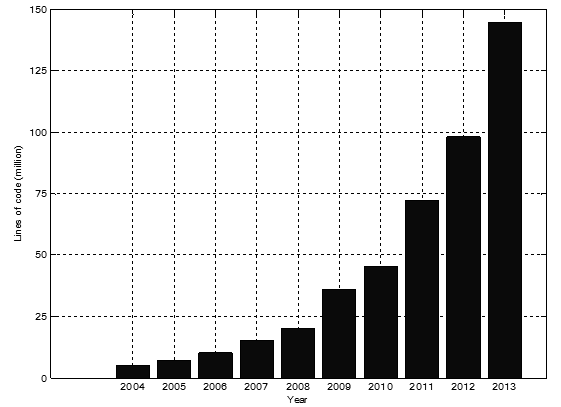
\includegraphics[width=\linewidth]{images_folder/Yearly-increase-in-automotive-software-complexity-shown-by-million-lines-of-code-of-1-ConvertImage.png}
    \caption{Yearly increase in automotive software complexity}
    \label{fig:yearlyincreas}
\end{figure}
Software development therefor faces new challenges, related to shorten development time, a high need of scalability  not only in the software but also in the development platforms, complex safety requirements and adaptability over continuously changing hardware.\\
Model based design has entered the automotive conversation because it can full fill the previously reported challenges. The model based approach brings two main characteristic to the table: on the one hand it gives a development platform which is component independent, therefor allowing for better integration through rapidly changing hardware, on the other hand makes the integration of new features not time depended. In this sense it recall a concept similar to Scurm, where changes are welcomed during the whole development process. in this case, with model based design, changes are welcomed during the whole life of the software.
\subsection{Model based design}
Model-Based Design provides a mathematical and visual approach to develop complex control and signal processing systems. It centers on the use of system models throughout the development process for design, analysis, simulation, automatic code generation and verification \cite{Mathworks}. The main features are abstraction and automation. As reported by \cite{modelbased} model based tackle complexity via abstraction and automation. Abstraction is achieved by the using suitable models of a software system, while automation is achieved by systematically transform these models into executable source code.\\
Engineers create a model to specify the behavior of an embedded system; the model, which consists of block diagrams, textual programs, and other graphical elements, is an executable specification that lets engineers run simulations to test ideas and verify designs throughout the development process. The main advantages are
\begin{itemize}
    \item The design can be tested, refined and retested throughout the development process, thus increasing product quality. Test and validation are done continuously rather than at the end of the process. Error can be found before hardware is required for testing
    \item Simplification of complex system, by providing a graphical design models simplify the creation of high complexity functions, especially when compared with hand code components. This advantage as it enhance and simplify communication inside the team, as it is easy to understand the models. 
    \item Embedded code can be generate automatically from the models. To adapt the model to different hardware there´s the need to adjust the compiler, not every single model. This allow for great adaptability to rapidly changing hardware. 
\end{itemize}
\subsection{From functions to c code or other type of artifacts}
\section{Ecu structure}
\subsection{Electrical ecu structure}
\subsection{Software ecu structure}
\section{Scons - build organization}

\cleardoublepage
\end{document}